% ----------
% A LaTeX template for course project reports
% 
% This template is modified from "Tech Report ala MIT AI Lab (1981)"
% 
% ----------
\documentclass[12pt, letterpaper, twoside]{article}
\usepackage{geometry}
\usepackage[utf8]{inputenc}
\usepackage[english]{babel}
\usepackage[runin]{abstract}
\usepackage{titling}
\usepackage{booktabs}
\usepackage{fancyhdr}
\usepackage{helvet}
\usepackage{csquotes}
\usepackage{graphicx}
\usepackage{blindtext}
\usepackage{parskip}
\usepackage{etoolbox}
\usepackage[export]{adjustbox}
\usepackage{float}

% preamble.tex

\geometry{letterpaper, top=2.2in, headheight=1.7in}
\date{}

\makeatletter

\def\fulltitle#1{\def\@fulltitle{#1}}
\def\runningtitle#1{\def\@runningtitle{#1}}
\def\runningauthor#1{\def\@runningauthor{#1}}
\def\affiliation#1{\def\@affiliation{#1}}
\def\department#1{\def\@department{#1}}
\def\memoid#1{\def\@memoid{#1}}
\def\theyear#1{\def\@theyear{#1}}
\def\mydate#1{\def\@mydate{#1}}

\runningtitle{How to write an effective report} % Short title
\author{Your name \and John Doe \and Jane Doe} % Full list of authors
\runningauthor{Your name et al.} % Short list of authors
\affiliation{Your University} % Affiliation e.g. University or Company
\department{Your Department} % Department or Office
\memoid{AI Memo 777} % ID of the tech report
\theyear{2018} % year of the tech report
\mydate{August 08, 2018} %the date

\def\displaymydate{\@mydate}
\def\displaytheyear{\@theyear}
\def\displaymemoid{\@memoid}
\def\displaydepartment{\@department}
\def\displayaffiliation{\@affiliation}
\def\displayrunningauthor{\@runningauthor}
\def\displayrunningtitle{\@runningtitle}

\makeatother

\makeatletter
\patchcmd{\@zfancyhead}{\fancy@reset}{\f@nch@reset}{}{}
\patchcmd{\@set@em@up}{\f@ncyolh}{\f@nch@olh}{}{}
\patchcmd{\@set@em@up}{\f@ncyolh}{\f@nch@olh}{}{}
\patchcmd{\@set@em@up}{\f@ncyorh}{\f@nch@orh}{}{}
\makeatother

% ----------
% fancyhdr setup
% ----------

\pagestyle{fancy}
\renewcommand{\headrulewidth}{0pt}

\fancypagestyle{firstpage}
{
    \fancyhf{}
    \fancyhead{%
        \begin{center}
            \textsc{\displayaffiliation}\\
            \textsc{\displaydepartment}
        \end{center}
        \vspace*{0.5in}
        \displaymemoid
        \hfill
        \displaymydate
    }
    \fancyfoot[L]{\footnotesize \textbf{\textsc{\displayaffiliation} -- \displaytheyear}}
}
\fancyhead[EL]{\small \displayrunningauthor}
\fancyhead[ER]{\small Page \thepage}
\fancyhead[OL]{\small Page \thepage}
\fancyhead[OR]{\small \displayrunningtitle}

\chead{}
\lfoot{}
\cfoot{}
\rfoot{}

% ----------

\providecommand{\keywords}[1]{\noindent \textbf{Keywords:} #1} % keywords definition

\renewcommand{\familydefault}{\sfdefault} % sans-serif font
\setlength{\parskip}{1em} % 1em skip between paragraphs
\abslabeldelim{:} % use colon after the run-in 'Abstract' word
\setlength{\parindent}{0pt} % no indentantion for first page 
\setlength{\abstitleskip}{-\absparindent} % this is because the abstract package sets \absparindent to \parindent

\pretitle{\Large \begin{center}}
\posttitle{\\[2ex] \Large \textbf{by}\end{center}}

% ----------
% Variables
% ----------

\title{\textbf{Econometrics 2 Course Project:\\Gravity Model in Iran-China Trade}} % Full title of your tech report
\runningtitle{Gravity model} % Short title
\author{Ali Asghari } % Full list of authors
\runningauthor{Ali Asghari.} % Short list of authors
\affiliation{Shahid Beheshti University} % Affiliation e.g. University or Company
\department{The Faculty of Economics and Political Science} % Department or Office
\memoid{Student ID: 98217011} % Project group ID that were shared with the class earlier.
\theyear{2022} % year of the tech report
\mydate{December, 2022} %the date


% ----------
% actual document
% ----------
\begin{document}
\maketitle



\vspace{2.5cm}

% Uncomment the following to add thanks.
% {\footnotesize
%     \noindent
%     Special thanks to \textbf{Person 1} and \textbf{Affiliation A} for financial support for this project.
% }

\thispagestyle{firstpage}

\pagebreak

% ----------
% End of first page
% ----------

\newgeometry{} % Redefine geometries (normal margins)

\section{Introduction}
\label{sec:intro}
The gravity model is a model used in international trade and attempts to explain the trade flow between two large economies is stronger than the trade flow between two smaller economies, and also economies that are closer to each other have more trades to each other than economies that are far from each other. The gravity equation was introduced in 1962 by Tinbergen in his book "Shaping the World Economy".

The gravity model has always existed in political circles as a comprehensive tool for analyzing various trade issues. The academic popularity of analyzing international trade based on gravity declined in the 1970s and 1980s, mainly because the gravity model can be extracted from almost any international trade model. The lack of a convincing and unambiguous basis in the field of microeconomics gave the gravity model a dual reputation: it may be a useful empirical tool, but from a theoretical point of view it is not satisfying. In the past twenty years, this model has returned to academic discussions with firmer foundations by people like Anderson and Bergstrand.\cite{Bergeijk(2014)}

The gravity model has a long history; many writers have referred to the flow between different places, and the "weight" of these places. Isard and Peck\cite{Isard and Peck (1954)}, based on theory and with the motivation to introduce multilateral trade and distance to the common tools of trade economists, empirically demonstrated the negative effect of distance on different modes of international and domestic trade. In fact, they come close to formulating gravity. But they use a different metaphor from physics to formulate their idea. In fact, Isard uses electric potential instead of Newtonian gravity. However, Isard had already envisioned many of the issues that gravity model researchers are engaging today; Because he uses cultural and political factors in his research. However, the first mathematical formulation and empirical application of this model was made by a group of Dutch economists led by Tinbergen, and they were the ones who really applied the modern gravity model in international trade.\cite{Tinbergen(1963)}Tinbergen was the supervisor of Linnemann's doctoral thesis\cite{Linnemann (1967)}, which became the standard reference for the original version of the gravity equation. The basic form of the gravity model can be shown as follows:
\[T_{ij}=X_{i\to j}+X_{j \to i}=X_{i \to j}+M_{i \to j}= X_{j \to i}+M_{j \to i}=M_{ i \to j}+M_{j \to i}\]
However, in this study, due to the availability of statistics on Iran's exports to China and Iran's imports from China, the sum of these two quantities, which existed in the central bank data, has been used. Iran's gross domestic product statistics from the Central Bank and China's gross domestic product statistics from World Bank data were used.

Therefore, the initial equation formed between the two countries will be as follows:
\[T_{Iran,China}=\frac{GDP_{Iran}^{\beta_{2}}GDP_{China}^{\beta_{3}}}{D_{Iran,China}^{\beta_{1}}}\]
Given the use of the OLS method for estimations and facilitating calculations, the above equation is transformed using the properties of the logarithm as follows:
\[Ln(T_{Iran,China})=-\beta_{1}Ln(D_{Iran,China})+{\beta_{2} Ln(GDP_{Iran}})+\beta_{3}Ln(GDP_{China})\]
In all exercises, the above equation was used as the main equation, and by substituting the following symbols for the above symbols, an attempt was made to simplify the equation:
\[TRADE=C+\beta_{2}China{\_}GDP+\beta_{3}Iran{\_}GDP\]

\section{Exercises}
\subsection{Partial Coefficients}
To show that the betas are partial regression coefficients, first we take the original regression model and regress the dependent variable which is the trade volume between Iran and China (which is introduced in the table with the name TRADE) on the explanatory variables China's Gross Domestic Product (China GDP) and Iran's Gross Domestic Product (Iran GDP). We then note the coefficient of the first explanatory variable (China's Gross Domestic Product).

    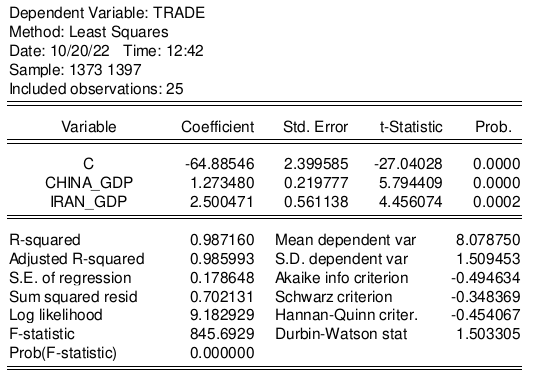
\includegraphics[width=.8\textwidth,height=.8\textwidth,keepaspectratio,center]{1.png} 

Next, while keeping Iran's Gross Domestic Product constant, we obtain the new model in the form of\(Y_{i}=b_{1}+b_{13}X_{3i}+e_{1i}\) in the regression. We then save the residual values (e) as a new variable.

    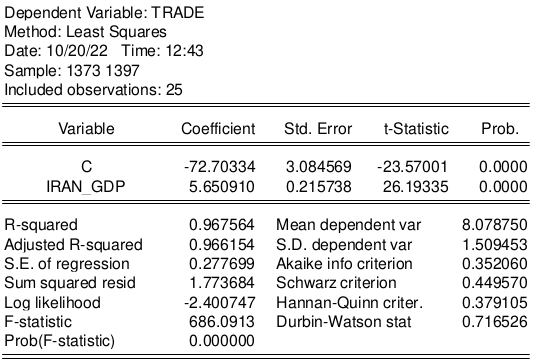
\includegraphics[width=.8\textwidth,height=.8\textwidth,keepaspectratio,center]{2.png}

Then taking \(X_{2i}\) as dependent variable ( China’s GDP) and regress it on Iran’s GDP and save the residuals as \(e_{2i}\)

    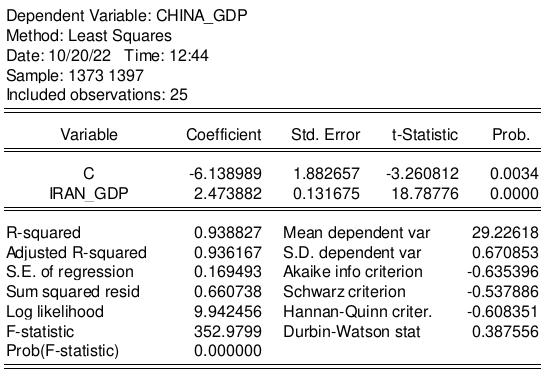
\includegraphics[width=.8\textwidth,height=.8\textwidth,keepaspectratio,center]{3.png}

Finally, we enter the first residual values as the dependent variable and the second residual values‬ as the explanatory variable in a new regression and perform the regression. According to the theory we expect that the regression coefficient of the explanatory variable will be the original regression coefficient

    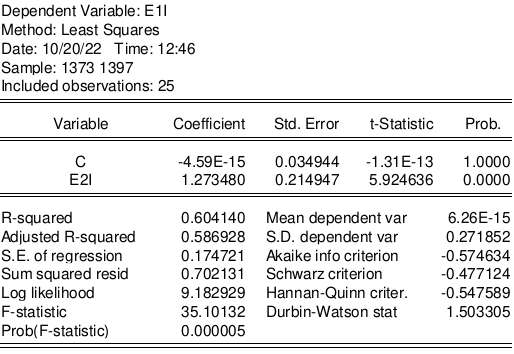
\includegraphics[width=.6\textwidth,height=.6\textwidth,keepaspectratio,center]{4.png}

we can see that the coefficients are the same
\[e_{2i}=\beta_{2}=1.273\]

\subsection{Comparing R squared}
We know that to compare \(R^2\) the values of two regression models with each other, the dependent variable of both models must be the same.
To do this, we define the following two regression models:
\begin{enumerate}
  \item The main regression model of the exercise which is as follows:
  \[ln(trade)=ln(China{\_}GDP)+ln(Iran{\_}GDP)+c\]
  \item The regression model in which the natural logarithm of the dependent variable is taken: 
    \[ln(ln(trade))=ln(ln(China{\_}GDP))+ln(Iran{\_}GDP))+c\]
\end{enumerate}
First we take the second regression model and observe that the value of R-squared is equal to 0.983 and we know that this value cannot be compared with the original regression model which is equal to 0.987.

To compare these two values, we first obtain the predicted values of the dependent variable of the second model (hats) then take the anti-logarithm of them and save them as the Fitted variable. Then we enter these values into a new regression model as the dependent variable and regress them on the explanatory variable which is the trade volume, which is the dependent variable of the first model. Now we can compare the obtained value, which is equal to 0.982, with the original one (0.987).

    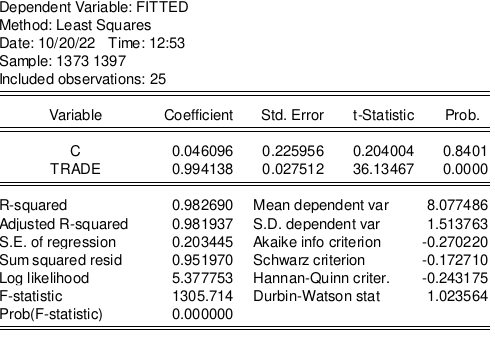
\includegraphics[width=.6\textwidth,height=.6\textwidth,keepaspectratio,center]{5.png}
        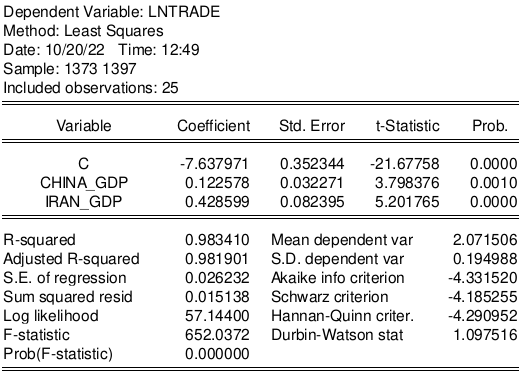
\includegraphics[width=.6\textwidth,height=.6\textwidth,keepaspectratio,center]{6.png}
\subsection{Define the AOV table based on R-squared}
with the use of Variance formula we can calculate the \(\sum_{}^{}Y_{i}^2\)
\[Var(y)=\frac{\sum_{}^{}Y_{i}^2}{n-1}\to1.5094^2=\frac{\sum_{}^{}Y_{i}^2}{24}\to\sum_{}^{}Y_{i}^2=54.6789\]
then with the help of R-squared we define the AOV table as below:
\begin{table}[ht]
\centering
\begin{tabular}{|l|l|l|l|}
\hline
MSS                                          & df     & SS                                                                                                & Source of the changes      \\ \hline {$\displaystyle\frac{53.9735}{2}=26.9867$} & 2      & {$\displaystyle R^2\sum y_{i}^2==53.9735$}        & Changes for the regression \\ \hline
{$\displaystyle \frac{0.7053}{22}=0.032$}   & N-3=22 & {$\displaystyle (1-R^2)\sum y_{i}^2==0.7053$} & Residuals                  \\ \hline
                                             & N-1=24 & {$\displaystyle \sum y_{i}^2=54.6789$}                                            & Sum                        \\ \hline
\end{tabular}
\end{table}


Now we want to determine the AOV table to evaluate the contribution of an additional variable. First, we estimate the model with only the first explanatory variable (China's GDP) and we get the following table:

    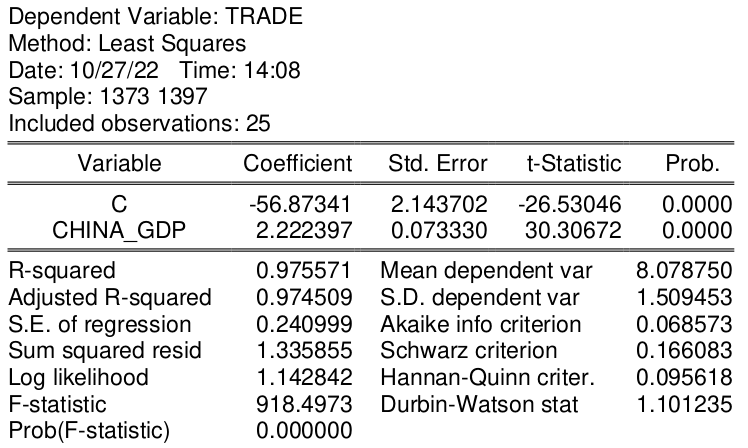
\includegraphics[width=.6\textwidth,height=.6\textwidth,keepaspectratio,center]{7.png}

Now we can create the AOV table based on the regression above:
\begin{table}[H]
\centering
\begin{tabular}{|l|l|l|l|}
\hline
MSS     & df & SS & \begin{tabular}[c]{@{}l@{}}Source of \\ the changes\end{tabular} \\ \hline
53.347  & 1  & {$\displaystyle Q_{1}=\hat{\beta_{12}}\sum x_{2}^2=53.347$}  & {$\displaystyle X_{2} \;ESS$}                                                                \\ \hline
0.6309  & 1  & {$\displaystyle Q_{2}=Q_{3}-Q_{1}$}  & {$\displaystyle X_{3} \;ESS$}                                                                \\ \hline
26.9886 & 2  & {$\displaystyle Q_{3}=\hat{\beta_{2}}\sum y_{i}x_{2i}+\hat{\beta_{3i}}\sum y_{i}x_{3i}=53.97$}  & {$\displaystyle X_{2},X_{3} \; ESS $}                                                                \\ \hline
0.032   & 22 & {$\displaystyle Q_{4}=Q_{5}-Q_{3}$}  & RSS                                                              \\ \hline
        & 24 & {$\displaystyle Q_{5}=\sum y_{i}^2=54.6827$}  & Sum                                                              \\ \hline
\end{tabular}
\end{table}
Now we can calculate F value:

\[F=\frac{\frac{Q_{2}}{df}}{\frac{Q_{4}}{df}}=19.71>F_{0.01,122}\]
It is observed that in the F-test, the obtained value is greater than the critical value, so the hypothesis that   \(\hat{\beta_{3}}\) is insignificant is rejected and it can be concluded that adding Iran's GDP variable to the model significantly increases the ESS and R-squared.

We can also manually compare the obtained table with the values that we get from the software, which also gives the same numbers in this comparison

    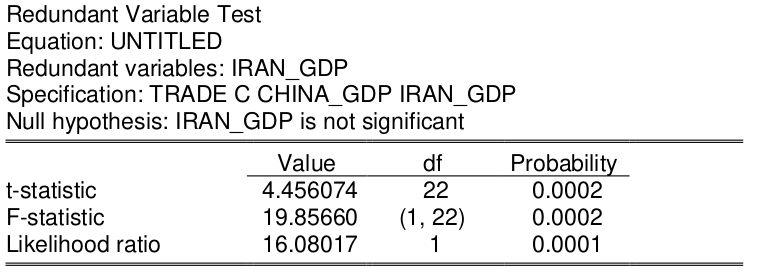
\includegraphics[width=.6\textwidth,height=.6\textwidth,keepaspectratio,center]{8.png}
        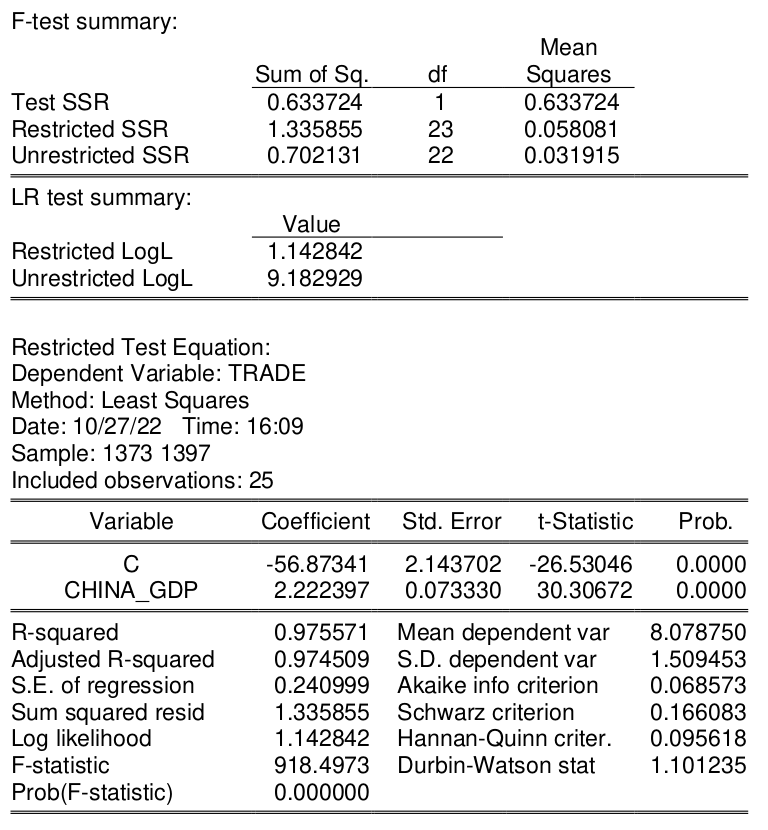
\includegraphics[width=.6\textwidth,height=.6\textwidth,keepaspectratio,center]{9.png}
\subsection{Heteroscedasticity tests}
First, we use the graphical method, to check if we can see any obvious heteroscedasticity. we plot the squared residuals versus the X's. According to the graphical method, heteroscedasticity is not observed in the variances.

        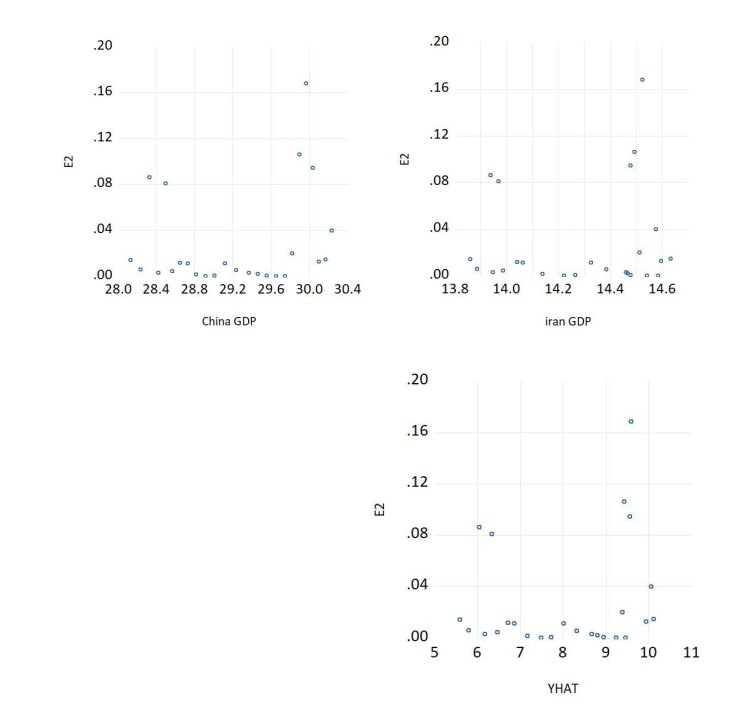
\includegraphics[width=.5\textwidth,height=.5\textwidth,keepaspectratio,center]{10.png}
We perform the Park test on the data and realize that the coefficients of the explanatory variables are significant while the C coefficient is not significant. This shows us that there is heteroscedasticity and there is no constant variance for the data.

        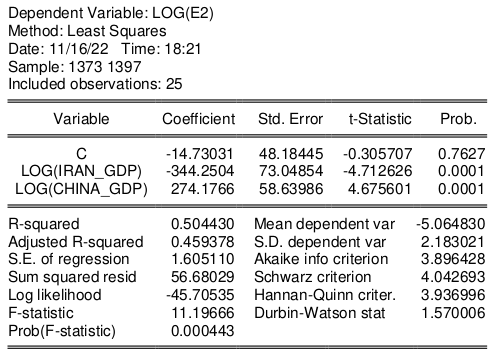
\includegraphics[width=.6\textwidth,height=.6\textwidth,keepaspectratio,center]{11.png}

Next, we perform the Glejser test\(\left|e_{i}  \right|=\beta_{1}+\beta_{2}X+v_{i}\) on the data and obtain significant coefficients for Iran's and China's GDP, which indicates heteroscedastic variances.

        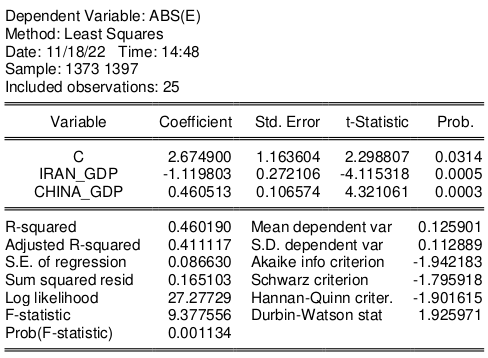
\includegraphics[width=.6\textwidth,height=.6\textwidth,keepaspectratio,center]{12.png}

Then, we perform the Glejser test \(\left|e_{i}  \right|=\beta_{1}+\beta_{2}\sqrt{X}+v_{i}\) on the data and find heteroscedasticity in the outputs.

        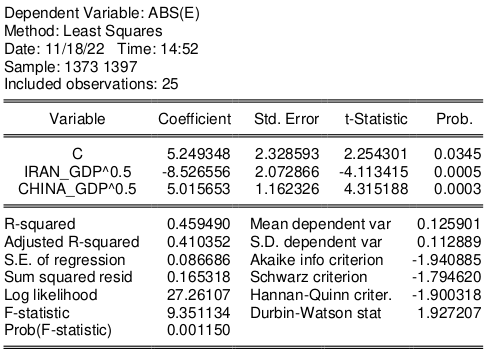
\includegraphics[width=.6\textwidth,height=.6\textwidth,keepaspectratio,center]{13.png}

We perform the Glejser test \(\left|e_{i}  \right|=\beta_{1}+\beta_{2}\frac{1}{X}+v_{i}\) and obtain significant coefficients and conclude heteroscedasticity.

        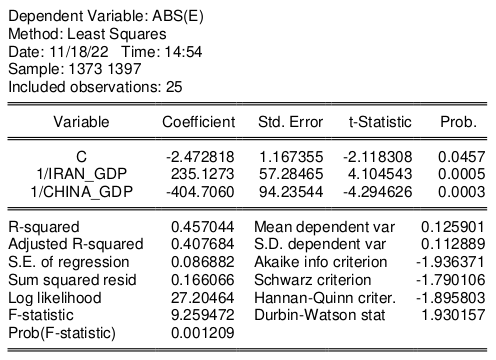
\includegraphics[width=.6\textwidth,height=.6\textwidth,keepaspectratio,center]{14.png}
We perform the \(\left|e_{i}  \right|=\beta_{1}+\beta_{2}\frac{1}{\sqrt{X}}+v_{i}\) test and still find heteroscedasticity.

        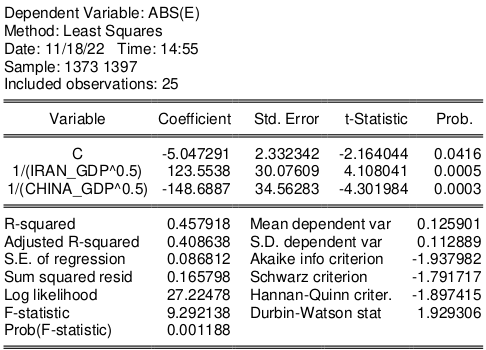
\includegraphics[width=.6\textwidth,height=.6\textwidth,keepaspectratio,center]{15.png}
\subsection{Autocorrelation}

First we want to see Autocorrelation with ploting the residuals. We plot the standardized residuals using Eviews:

        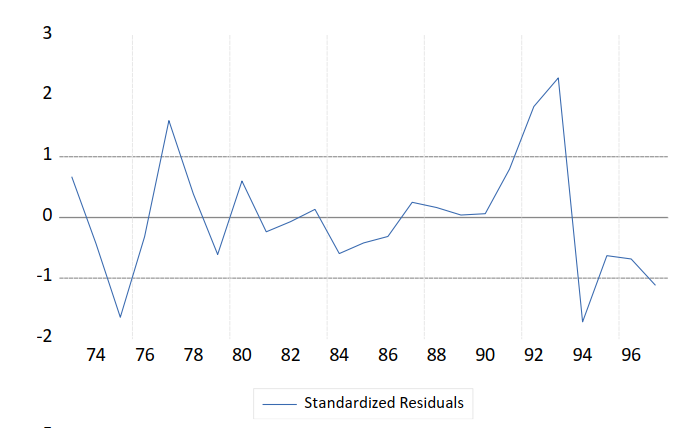
\includegraphics[width=.6\textwidth,height=.6\textwidth,keepaspectratio,center]{16.png}
        
We can also scatter residuals and their lags as below:

        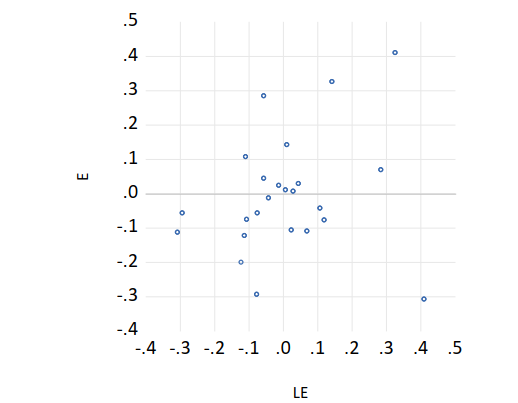
\includegraphics[width=.6\textwidth,height=.6\textwidth,keepaspectratio,center]{17.png}
        
We can guess from the figures above that we might have autocorrelation.

Now to be sure of autocorrelation we check Durbin–Watson stats.

        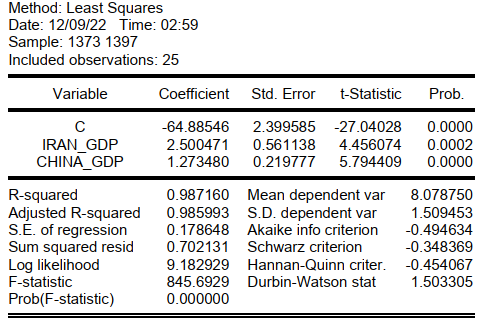
\includegraphics[width=.6\textwidth,height=.6\textwidth,keepaspectratio,center]{18.png}
        
We see that the stats is in the inconclusive area.

Now we use LM test and get the following results:

        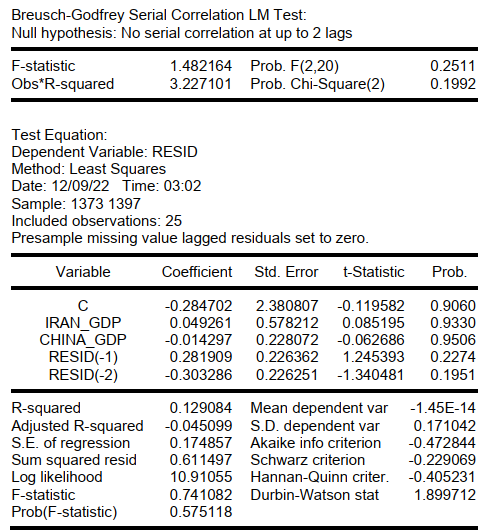
\includegraphics[width=.6\textwidth,height=.6\textwidth,keepaspectratio,center]{19.png}

        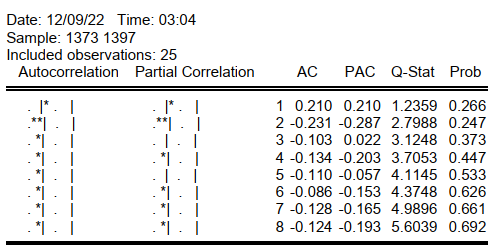
\includegraphics[width=.6\textwidth,height=.6\textwidth,keepaspectratio,center]{20.png}
        
With looking at the probe values we can claim that we do not have autocorrelation.

\subsection{Omitted variable and redundant variable}

In this exercise, we want to check how omitted variable can change the model. To test it, first we estimate the model without China’s GDP

        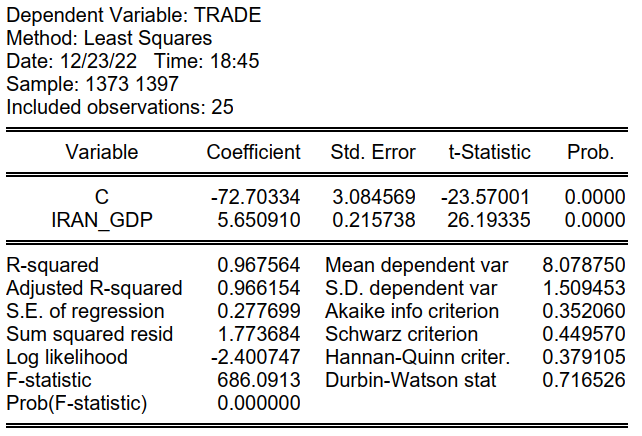
\includegraphics[width=.6\textwidth,height=.6\textwidth,keepaspectratio,center]{21.png}
        
Then we run omitted variable test

        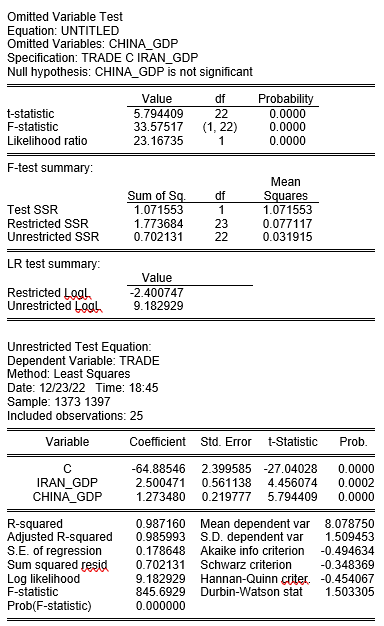
\includegraphics[width=.8\textwidth,height=.8\textwidth,keepaspectratio,center]{22.png}
        
We can clearly see that China’s GDP omitted variable lead to the incorrect model with omitted variable bias

Now we want to test how adding the trend variable to the model change the model. So we create and add the trend to the model and estimate the model as below:

        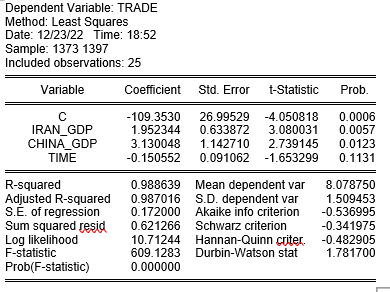
\includegraphics[width=.6\textwidth,height=.6\textwidth,keepaspectratio,center]{23.png}
        
Now we test redundant variable using Eviews

        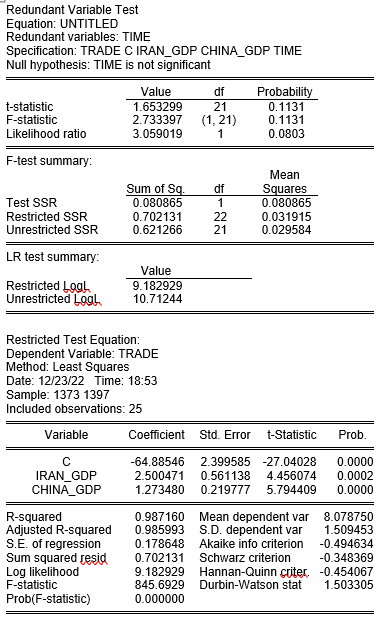
\includegraphics[width=.8\textwidth,height=.8\textwidth,keepaspectratio,center]{24.png}
        
We can see that time variable is not meaningful.

\subsection{Normality of the residuals}

At last, we want to check the normality of residuals using Jarque–Bera test.

        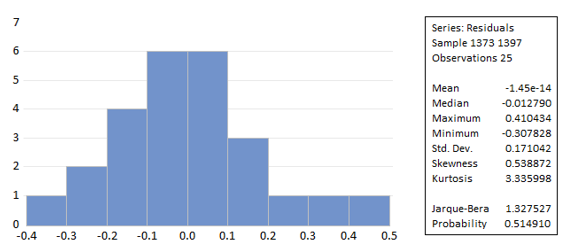
\includegraphics[width=.6\textwidth,height=.6\textwidth,keepaspectratio,center]{25.png}
        
From the results, we can assume the residual has a normal distribution.


% Uncomment following to add an acknowledgement section
% \section*{Acknowledgements}

% Thanks again to \textbf{Person 1} and \textbf{Affiliation A} for their financial support.
\pagebreak
% ----------
% Bibliography
% ----------

\begin{thebibliography}{9}
\bibitem{Isard and Peck (1954)}
Isard, W., & Peck, M. J. (1954). Location theory and international and interregional trade theory. The Quarterly Journal of Economics, 68(1), 97. https://doi.org/10.2307/1881920.

\bibitem{Linnemann (1967)}
Sawyer, J. A. (1967). An Econometric Study of International Trade Flows. By Hans Linnemann. Amsterdam: North-Holland Publishing Company. 1966. Pp. xiv, 234. The Canadian Journal of Economics and Political Science, 33(4), 633–634. https://doi.org/10.2307/140051

\bibitem{Tinbergen(1963)}
Tinbergen, J. (1963). Shaping the world economy. The International Executive, 5(1), 27–30. https://doi.org/10.1002/tie.5060050113
\bibitem{Bergeijk(2014)}
Van Bergeijk, P. A., & Brakman, S. (2014). The gravity Model in International Trade: Advances and applications. http://ci.nii.ac.jp/ncid/BB18037384


\end{thebibliography}

\end{document}

% ----------
